\documentclass[a4paper]{article}

\usepackage[top=1.2in, bottom=1.2in, left=1in, right=1in]{geometry}
\usepackage{fancyvrb, graphicx, hyperref, minted}
\usepackage[T1]{fontenc}

\hypersetup{colorlinks=true, linkcolor=black}

\title{Hardware Design and Implementation of LC2K Multiple Cycle Datapath and Controller}
\author{Rijun Cai\\12348003}

\begin{document}
\maketitle

\section{Objective}
The objective of this laboratory is to design a LC-2K processor with multiple cycle datapath using VHDL hardware description language and to simulate the execution of the instructions in machine language in ModelSim.

\section{Laboratory Tasks}
\begin{itemize}
    \item Design a multiple cycle datapath for LC2K ISA
    \item Design a FSM controller for this datapath
    \item Design the components of the datapath and the controller in VHDL language 
    \item Connect the components to form a whole VHDL model of the LC2K processor
    \item Simulate the execution of each instruction of LC2K ISA in ModelSim
\end{itemize}

\section{Designing Datapath}
We use the LC2K multiple cycle datapath in Figure~\ref{fig:datapath} from our lecture.
\begin{figure}[ht!]
    \center
    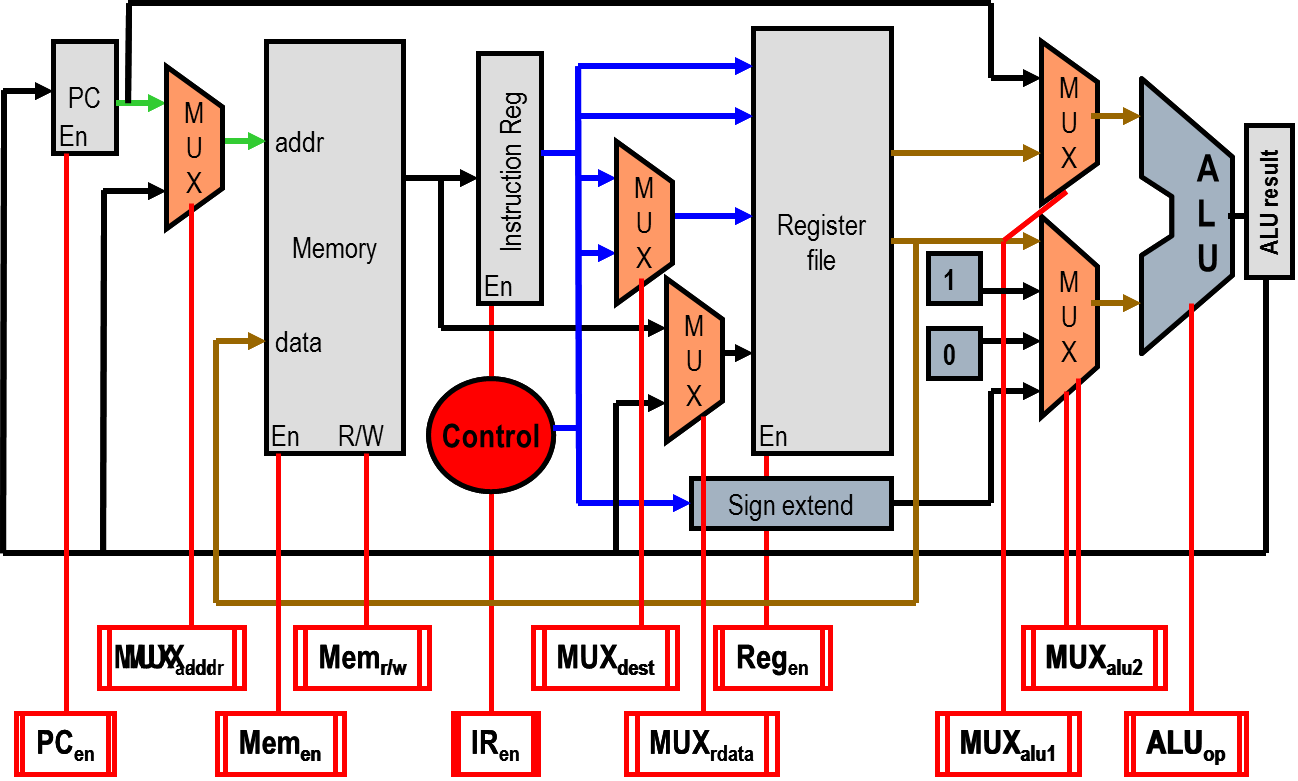
\includegraphics[scale=0.7]{datapath}
    \caption{Datapath}\label{fig:datapath}
\end{figure}
All element parts in this datapath are triggered by high voltage level of control signals except that the ALU result register, the register file and the memory are triggered by rising edge of the clock. At very first, all elements may he initialized and disabled.

\section{Designing Controller}
In the following, I will discuss the execution of the most important instructions within the datapath in detail. The execution of each instruction within the datapath consists of several cycles. The lines highlighted blue indicates the activated path in that cycle. All LC2K instructions have the format such as follows:
\begin{verbatim}
opcode RegA RegB desReg
opcode RegA RegB offset
opcode RegA RegB
opcode
\end{verbatim}

\subsection{FET0}\label{fec0}
Get instruction from the memory into the IR register. All instruction execution in this cycle is the same. See Figure~\ref{fig:fet0}.
\begin{figure}[ht!]
    \center
    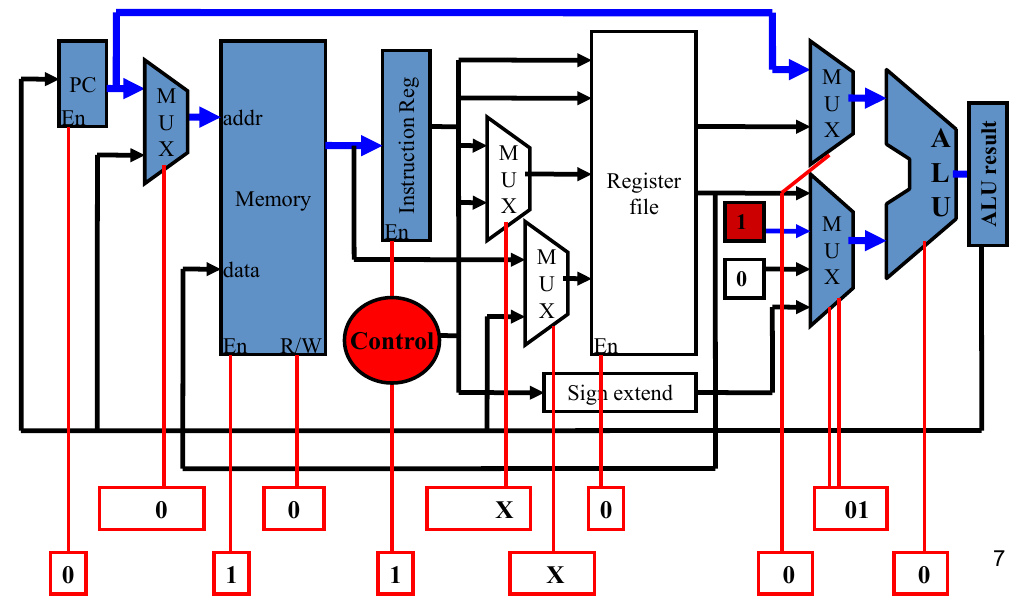
\includegraphics[scale=0.4]{fet0}
    \caption{FET0}\label{fig:fet0}
\end{figure}

\subsection{DEC1}\label{dec1}
When the rising edge of the CLK arrives, the instruction is stored in the IR and the PC + 1 is stored in the ALU Result Register.
In this state, the ``\verb|next state|'' output of the FSM is \verb|UNKNOWN|, which indicates that the next state of the FSM is
determined by an extra logic circuit, which calculates the next state of the FSM according to the instruction.
See Figure~\ref{fig:dec1}.
\begin{figure}[ht!]
    \center
    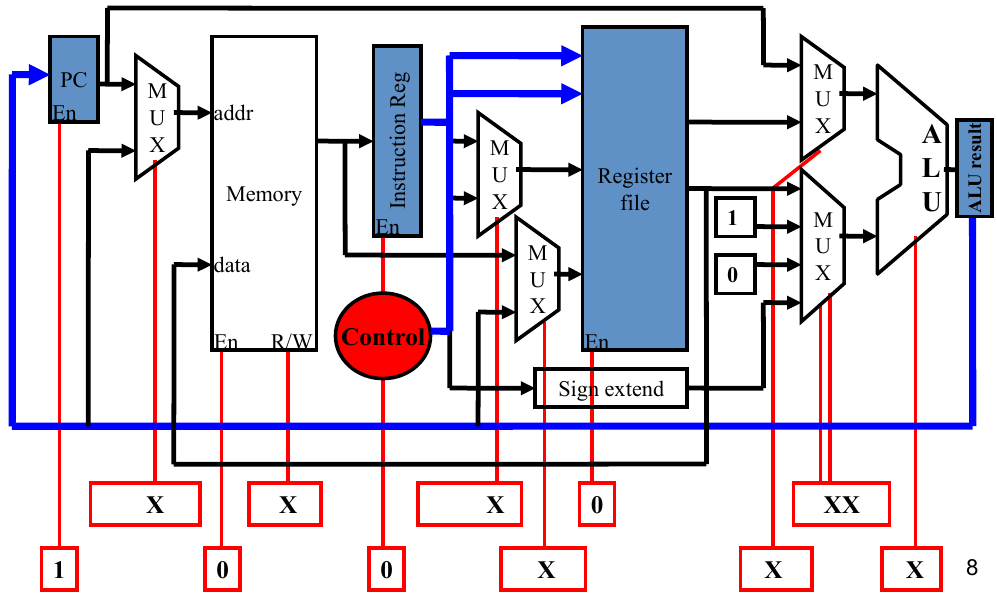
\includegraphics[scale=0.4]{dec1}
    \caption{DEC1}\label{fig:dec1}
\end{figure}

\subsection{ADD2}\label{add2}
In this cycle, \verb|RegA + RegB| is calculated by the ALU and the result is stored in the ALU Result Register at the end of this
cycle. See Figure~\ref{fig:add2}.
\begin{figure}[ht!]
    \center
    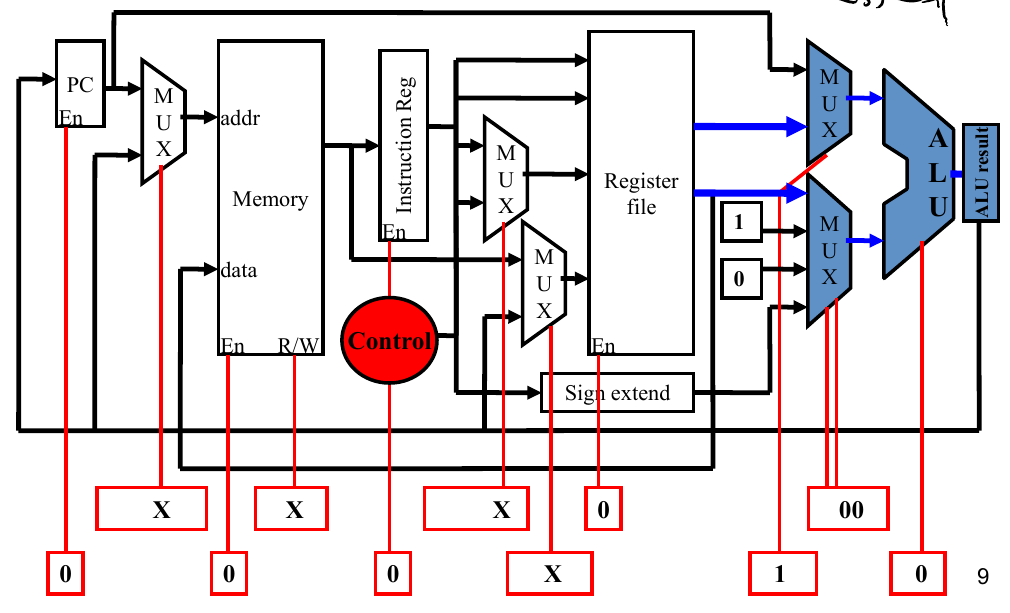
\includegraphics[scale=0.4]{add2}
    \caption{ADD2}\label{fig:add2}
\end{figure}

\subsection{ADD3}\label{add3}
In this cycle, the result of the ALU is stored in \verb|desReg|. The FSM returns to~\nameref{fec0} after this cycle.
See Figure~\ref{fig:add3}.
\begin{figure}[ht!]
    \center
    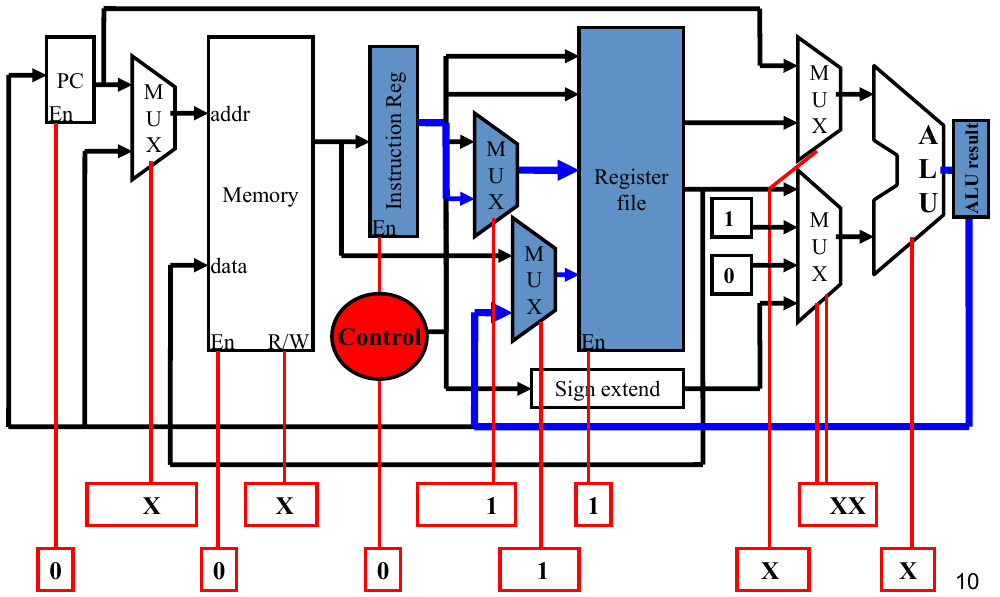
\includegraphics[scale=0.4]{add3}
    \caption{ADD3}\label{fig:add3}
\end{figure}

\subsection{NAND4}
This cycle is almost the same as~\nameref{add2} except that \verb|ALUop| is \verb|1| so that the ALU will do the NAND calculation
instead of the ADD calculation.

\subsection{NAND5}
This cycle is exactly the same as~\nameref{add3}.

\subsection{LW6}
The address of the data to be accessed is calculated in this cycle. The result is stored in the ALU Result Register.
See Figure~\ref{fig:lw6}.
\begin{figure}[ht!]
    \center
    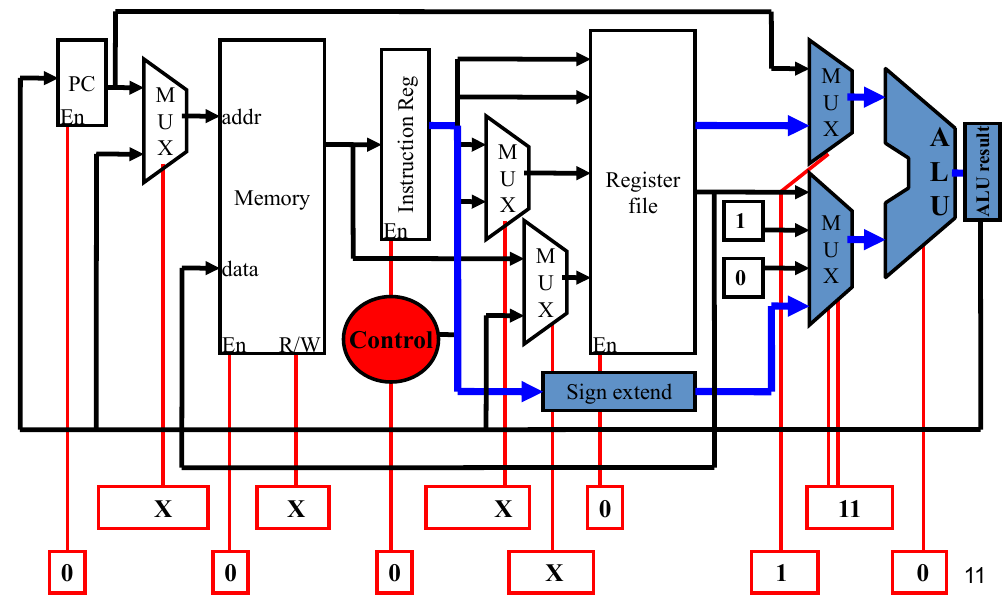
\includegraphics[scale=0.4]{lw6}
    \caption{LW6}\label{fig:lw6}
\end{figure}

\subsection{LW7}
The address calculated in the previous cycle is sent to the memory and then the memory output the desired data.
See Figure~\ref{fig:lw7}.
\begin{figure}[ht!]
    \center
    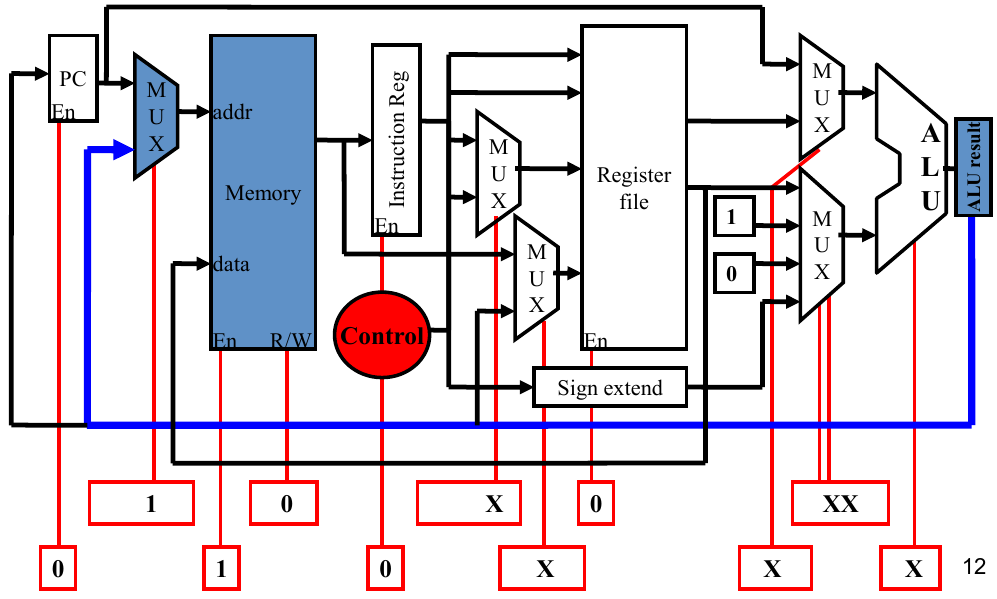
\includegraphics[scale=0.4]{lw7}
    \caption{LW7}\label{fig:lw7}
\end{figure}

\subsection{LW8}
The data from the memory are eventually stored in \verb|desReg| in this cycle. The FSM returns to~\nameref{fec0} after this cycle.
See Figure~\ref{fig:lw8}.
\begin{figure}[ht!]
    \center
    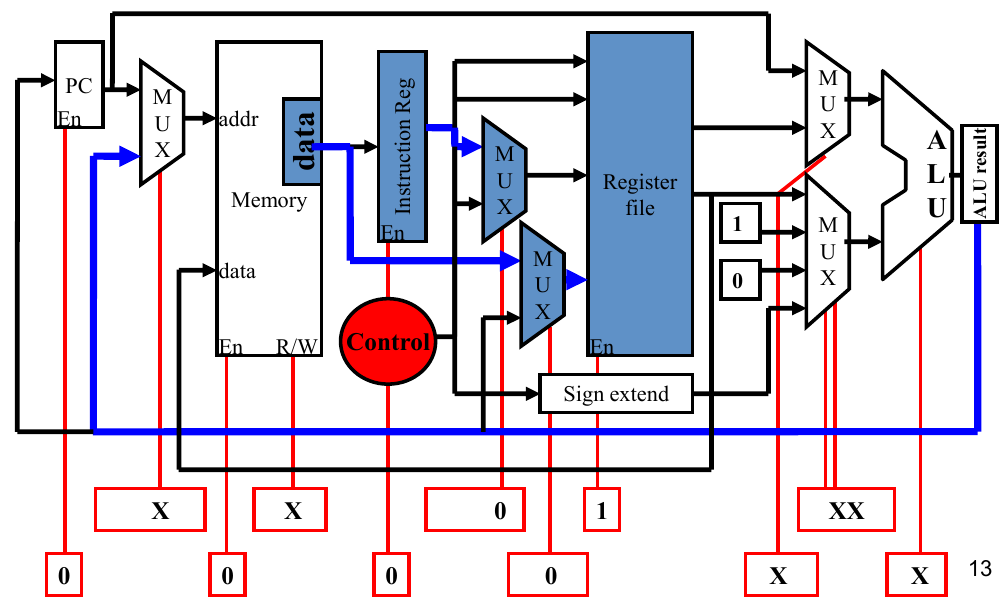
\includegraphics[scale=0.4]{lw8}
    \caption{LW8}\label{fig:lw8}
\end{figure}

\subsection{SW9}
In this cycle, the destination address is calculated by the ALU\@.

\subsection{SW10}
In this cycle, the data of \verb|RegB| are sent to the memory data input port, and are stored in the desired location at the end
of this cycle then the FSM returns to~\nameref{fec0}.

\subsection{BEQ11}
The address to which the CPU is going to branch is calculated in this cycle. See Figure~\ref{fig:beq11}.
\begin{figure}[ht!]
    \center
    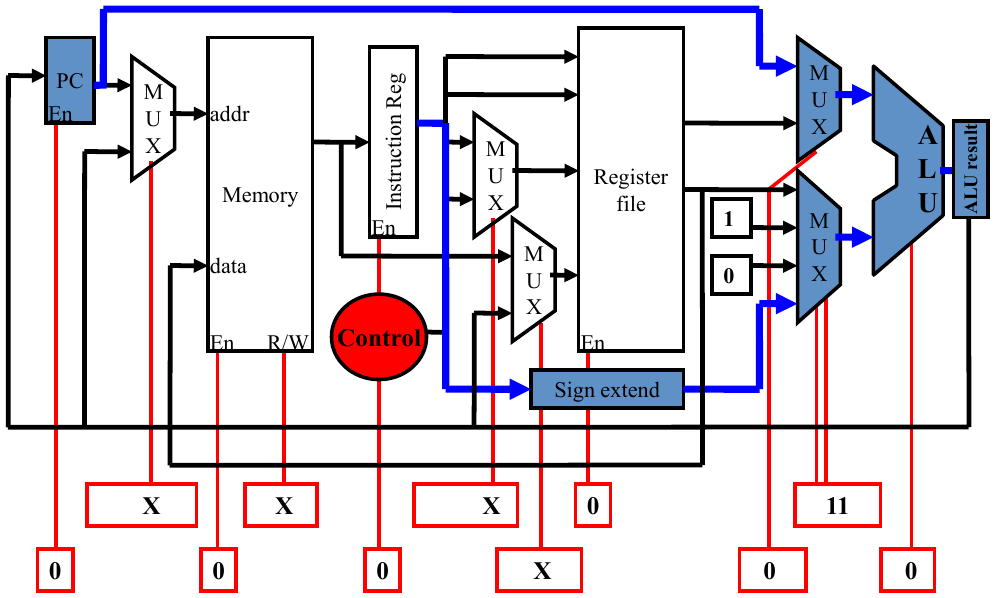
\includegraphics[scale=0.4]{beq11}
    \caption{BEQ11}\label{fig:beq11}
\end{figure}

\subsection{BEQ12}
In this cycle, the data of \verb|RegA| and \verb|RegB| are sent to the ALU and the equality of them are tested. \verb|PCen| is
controlled by an extra logic circuit that takes \verb|eq?| as an input. So when \verb|eq?| is \verb|1|, the PC Register is enable
then the CPU will branch to the desired address. See Figure~\ref{fig:beq12}.
\begin{figure}[ht!]
    \center
    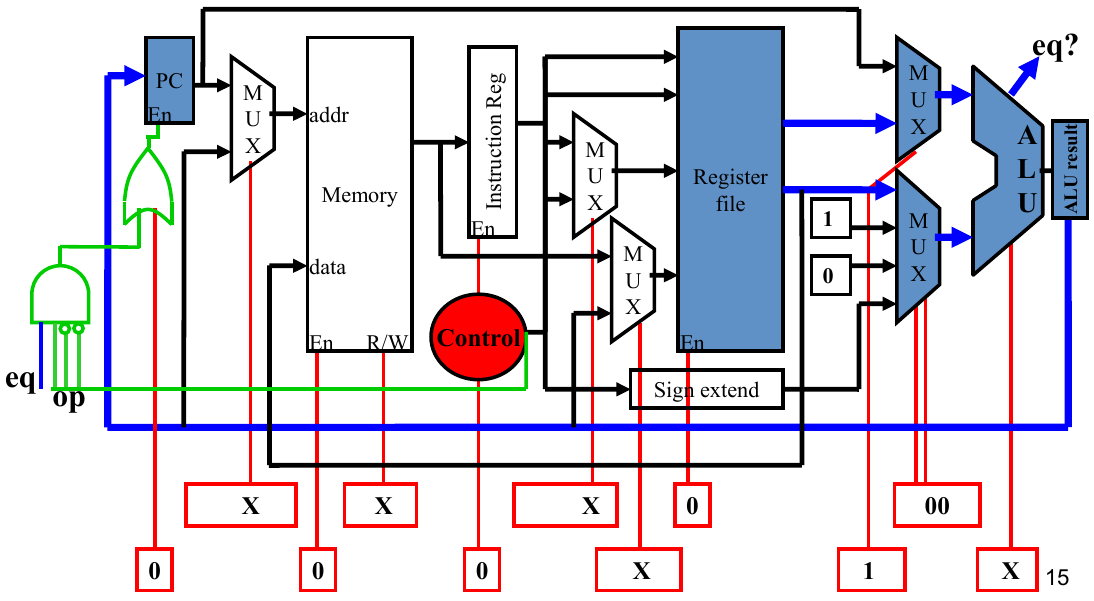
\includegraphics[scale=0.4]{beq12}
    \caption{BEQ12}\label{fig:beq12}
\end{figure}

\subsection{JALR13}
In this cycle, \verb|PC + 1|, which is calculated in \nameref{dec1}, is stored in the ALU Result Register.

\subsection{JALR14}
In this cycle, \verb|PC + 1| is stored in \verb|RegB|, then the data of \verb|RegA| is sent to the ALU and added with \verb|0|.

\subsection{JALR15}
In this cycle, the destination address, which is stored in the ALU Result Register in the previous cycle, is sent
to the PC register.

\section{Component Implementation in VHDL}
Please refer to the source code.

\section{Verifying Component in ModelSim}
\subsection{ALU}
\begin{description}
    \item[Add] See Figure~\ref{fig:alu_add}.

        \begin{figure}[ht!]
            \center
            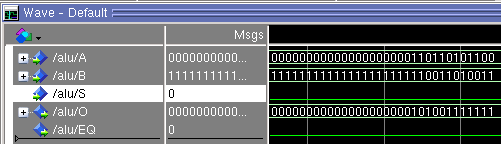
\includegraphics[scale=0.6]{alu_add}
            \caption{ALU Add}\label{fig:alu_add}
        \end{figure}

    \item[Nand] See Figure~\ref{fig:alu_nand}.

        \begin{figure}[ht!]
            \center
            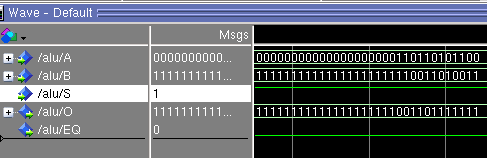
\includegraphics[scale=0.6]{alu_nand}
            \caption{ALU Nand}\label{fig:alu_nand}
        \end{figure}
\end{description}

\subsection{Multiplexer}
\begin{description}
    \item[2-to-1 Multiplexer] See Figure~\ref{fig:mux2}.

        \begin{figure}[ht!]
            \center
            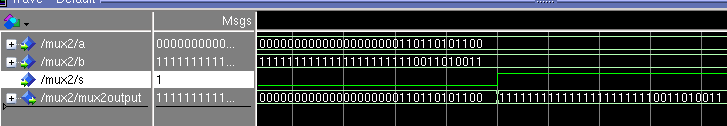
\includegraphics[scale=0.6]{mux2}
            \caption{2-to-1 Multiplexer}\label{fig:mux2}
        \end{figure}

    \item[4-to-1 Multiplexer] See Figure~\ref{fig:mux4}.

        \begin{figure}[ht!]
            \center
            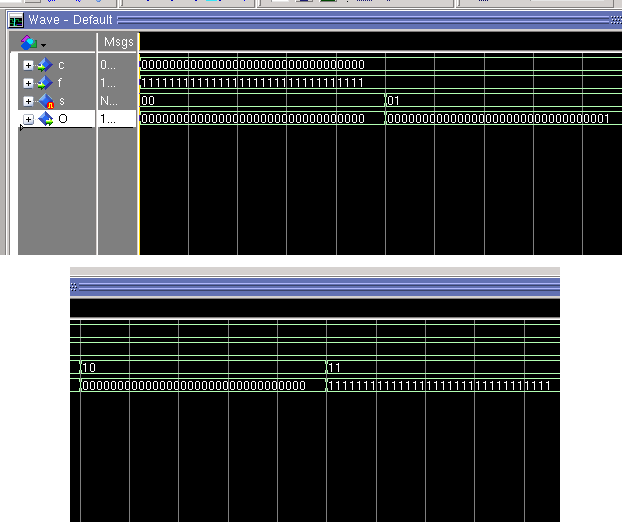
\includegraphics[scale=0.6]{mux4}
            \caption{4-to-1 Multiplexer}\label{fig:mux4}
        \end{figure}
\end{description}

\section{Describing Top Level Design in VHDL}
Please refer to the source code.

\section{Simulating the Whole System}
For convenience, I wrote a testing framework so that I didn't have to set the \verb|CLK| and \verb|RST| manually every time.
\begin{minted}[linenos]{vhdl}
library IEEE;
use IEEE.std_logic_1164.all;

entity TESTBOARD is
    port(
            PC: out STD_LOGIC_VECTOR (31 downto 0);
            IR: out STD_LOGIC_VECTOR (31 downto 0)
        );
end TESTBOARD;

architecture STR of TESTBOARD is

    component LC2K
        port(
                rst: in  STD_LOGIC;
                clk: in  STD_LOGIC;
                outPC: out std_logic_vector (31 downto 0);
                outMem: out std_logic_vector (31 downto 0);
                outIR: out std_logic_vector (31 downto 0);
                outRF1: out std_logic_vector (31 downto 0);
                outRF2: out std_logic_vector (31 downto 0);
                inALU1: out std_logic_vector (31 downto 0);
                inALU2: out std_logic_vector (31 downto 0);
                outALU: out std_logic_vector (31 downto 0);
                outp: out std_logic_vector (31 downto 0)
            );
    end component;

    constant period : time := 25 ns;

    signal rst : STD_LOGIC;
    signal clk : STD_LOGIC;
    signal outMem: std_logic_vector (31 downto 0);
    signal outRF1: std_logic_vector (31 downto 0);
    signal outRF2: std_logic_vector (31 downto 0);
    signal inALU1: std_logic_vector (31 downto 0);
    signal inALU2: std_logic_vector (31 downto 0);
    signal outALU: std_logic_vector (31 downto 0);
    signal outp: std_logic_vector (31 downto 0);

begin
    RSTprocess : process
    begin
        rst <= '1';
        wait for period * 2;
        rst <= '0';
        wait;
    end process RSTprocess;

    CLKprocess : process
    begin
        clk <= '0';
        wait for period;
        clk <= '1';
        wait for period;
    end process CLKprocess;

    U_CPU : LC2K port map (rst, clk, PC, outMem, IR, outRF1, outRF2,
        inALU1, inALU2, outALU, outp);

end STR;
\end{minted}

Besides, I also wrote a Python script to automatically convert machine codes (generated by \verb|assemble| in Lab 1) to
memory presentations in VHDL so that I didn't have to convert the machine codes to binary presentations and fill in the
memory's VHDL code manually every time.

\begin{minted}[linenos]{python}
#!/usr/bin/env python2

buf = []
try:
    while True:
        x = input()
        if not (-2 ** 31 <= x < 2 ** 31):
            break
        buf.append(x)
except (EOFError, TypeError):
    pass

for addr, ins in enumerate(buf):
    if ins >= 0:
        print 'regs(%d) <= "%s";' % (addr,
                bin(ins)[2:].rjust(32, '0'))
    else:
        print 'regs(%d) <= "%s";' % (addr,
                bin((1 << 32) + ins)[2:])
\end{minted}

\subsection{Test Case 1: Basic Test}

Assembly code:

\begin{minted}[linenos]{gas}
        lw      0       1       five    load reg1 with 5 (symbolic address)
        lw      1       2       3       load reg2 with -1 (numeric address)
start   add     1       2       1       decrement reg1
        beq     0       1       2       goto end of program when reg1 == 0
        beq     0       0       start   go back to the beginning of the loop
        noop
done    halt                            end of program
five    .fill   5
neg1    .fill   -1
stAddr  .fill   start                   will contain the address of start (2)
\end{minted}

Assemble and convert the code.

\begin{minted}{console}
$ ./assemble basic_test.asm basic_test.mc
$ ./convert_to_vhdl_mem.py < basic_test.mc > basic_test.mem
\end{minted}

Then copy and paste the content of \verb|basic_test.mem| to \verb|TestMem.vhdl|. Now test it in ModelSim.

The wave graph is shown in Figure~\ref{fig:wav_test1}.
\begin{figure}[ht!]
    \center
    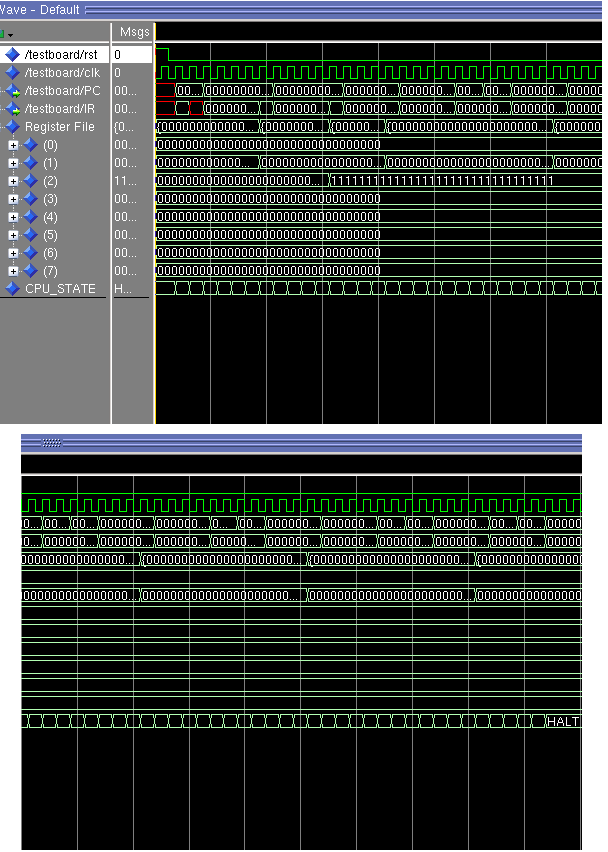
\includegraphics[scale=0.5]{wav_test1}
    \caption{Wave Graph of Test 1}\label{fig:wav_test1}
\end{figure}

And the final state of the register file is shown in Figure~\ref{fig:reg_test1}.
\begin{figure}[ht!]
    \center
    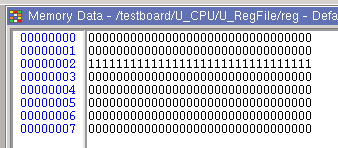
\includegraphics[scale=0.6]{reg_test1}
    \caption{Final State of the Register File in Test 1}\label{fig:reg_test1}
\end{figure}

\subsection{Test Case 2: Factorial Function}

Assembly code:

\begin{minted}[linenos]{gas}
init        lw      0   1   n
            lw      0   3   const+1
            lw      0   7   sp
            lw      0   4   const-2
            add     7   4   7
loop        beq     1   2   after-loop
            lw      0   4   const+1
            add     2   4   2
            sw      7   1   1
            sw      7   2   2
            add     0   3   1
            lw      0   4   mul-addr
            jalr    4   6
            lw      7   2   2
            lw      7   1   1
            beq     0   0   loop
after-loop  halt
mul         lw      0   4   const-2
            add     7   4   7
            sw      7   6   2
            sw      7   5   1
            add     0   0   3
            lw      0   5   mul-mask
            lw      0   6   mul-checker
mul-iter    nand    2   5   4
            beq     4   6   mul-skip
            add     3   1   3
mul-skip    add     5   5   5
            beq     5   0   mul-finish
            add     1   1   1
            beq     0   0   mul-iter
mul-finish  lw      7   5   1
            lw      7   6   2
            lw      0   4   const+2
            add     7   4   7
            jalr    6   4
const-2     .fill   -2
const+1     .fill   1
const+2     .fill   2
sp          .fill   255
mul-addr    .fill   mul
mul-mask    .fill   1
mul-checker .fill   -1
n           .fill   10
\end{minted}

The final state of the register file is shown in Figure~\ref{fig:reg_test2}.
\begin{figure}[ht!]
    \center
    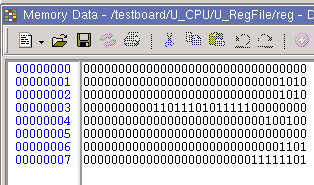
\includegraphics[scale=0.6]{reg_test2}
    \caption{Final State of the Register File in Test 2}\label{fig:reg_test2}
\end{figure}

\subsection{Test Case 3: k-Combinations of N}

Assembly code:

\begin{minted}[linenos]{gas}
init        lw      0   1   n
            lw      0   2   r
            lw      0   7   init-sp
            lw      0   4   comb-addr
            jalr    4   6
            halt
comb        beq     2   0   basic-sit
            beq     1   2   basic-sit
            lw      0   4   const-4
            add     7   4   7
            sw      7   6   4           save the return address
            sw      7   2   3           save R2(r) (as a local variable)
            sw      7   1   2           save R1(n) (as a local variable)
            lw      0   4   const-1
            add     1   4   1
            lw      0   4   comb-addr
            jalr    4   6
            sw      7   3   1           save C(n - 1, r) to stack
            lw      0   4   const-1
            lw      7   1   2           get local variable n
            lw      7   2   3           get local variable r
            add     1   4   1
            add     2   4   2
            lw      0   4   comb-addr
            jalr    4   6
            lw      7   4   1
            add     3   4   3           calulate C(n - 1, r - 1) + C(n - 1, r)
            lw      7   6   4           restore R6
            lw      0   4   const+4
            add     7   4   7
            jalr    6   4
basic-sit   lw      0   3   const+1
            jalr    6   4
init-sp     .fill   255
const+1     .fill   1
const+4     .fill   4
const-1     .fill   -1
const-4     .fill   -4
comb-addr   .fill   comb
n           .fill   7
r           .fill   3
\end{minted}

The final state of the register file is shown in Figure~\ref{fig:reg_test3}.
\begin{figure}[ht!]
    \center
    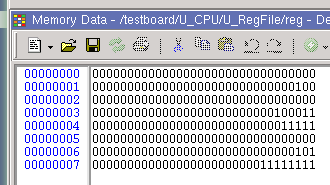
\includegraphics[scale=0.6]{reg_test3}
    \caption{Final State of the Register File in Test 3}\label{fig:reg_test3}
\end{figure}

For more test cases, please refer to the source code.

\section{Conclusion and Discussion}

In the simulation, the final states of the register file are identical to those of \verb|simulate| in Lab 2 for all test cases.
So it can be inferred that the CPU works as expected.

During the designing process, I noticed that the register file is not triggered by clock edge and the memory is asynchronous,
which may require more states in the FSM to ensure the register file and the memory work stably. But I don't want to add more
states to the FSM, so I change the designs of the register file and the memory. With the synchronous memory and register file
that triggered by clock edge, the CPU do not need extra states to perform the write operations. But I haven't made good use
of this feature by now, so the CPU can be optimized further.

\section{Sum-up}
In this experiment, I implemented a LC2K CPU with multiple cycle datapath. Through this, I came to know more about the
underlying details of how the CPU work, which is indispensable in designing high-performance programs.

\end{document}
